\begin{figure}[h]
     \centering
     \begin{subfigure}[b]{0.49\textwidth}
         \centering
         \includesvg[width=0.99\textwidth]{figures/results_wPCC_VCT.drift_angle_X.svg}
        \caption{Surge.}
        \label{fig:drift_angle_X}
     \end{subfigure}
     \hfill
     \begin{subfigure}[b]{0.49\textwidth}
         \centering
         \includesvg[width=0.99\textwidth]{figures/results_wPCC_VCT.drift_angle_Y.svg}
        \caption{Sway.}
        \label{fig:drift_angle_Y}
     \end{subfigure}
     \vfill
     \begin{subfigure}[b]{\textwidth}
         \centering
         \includesvg{figures/results_wPCC_VCT.drift_angle_N.svg}
        \caption{Yawing moment.}
        \label{fig:drift_angle_N}
     \end{subfigure}
    \caption{Overshoot angles from the wPCC experiments and simulations.}
    \label{fig:overshoots_wPCC}
\end{figure}


The flow from the port dagger board hits the starboard rudder for 15 degrees drift angle as shown in \autoref{fig:streamlines15}.
\begin{figure}[h]
    \centering
    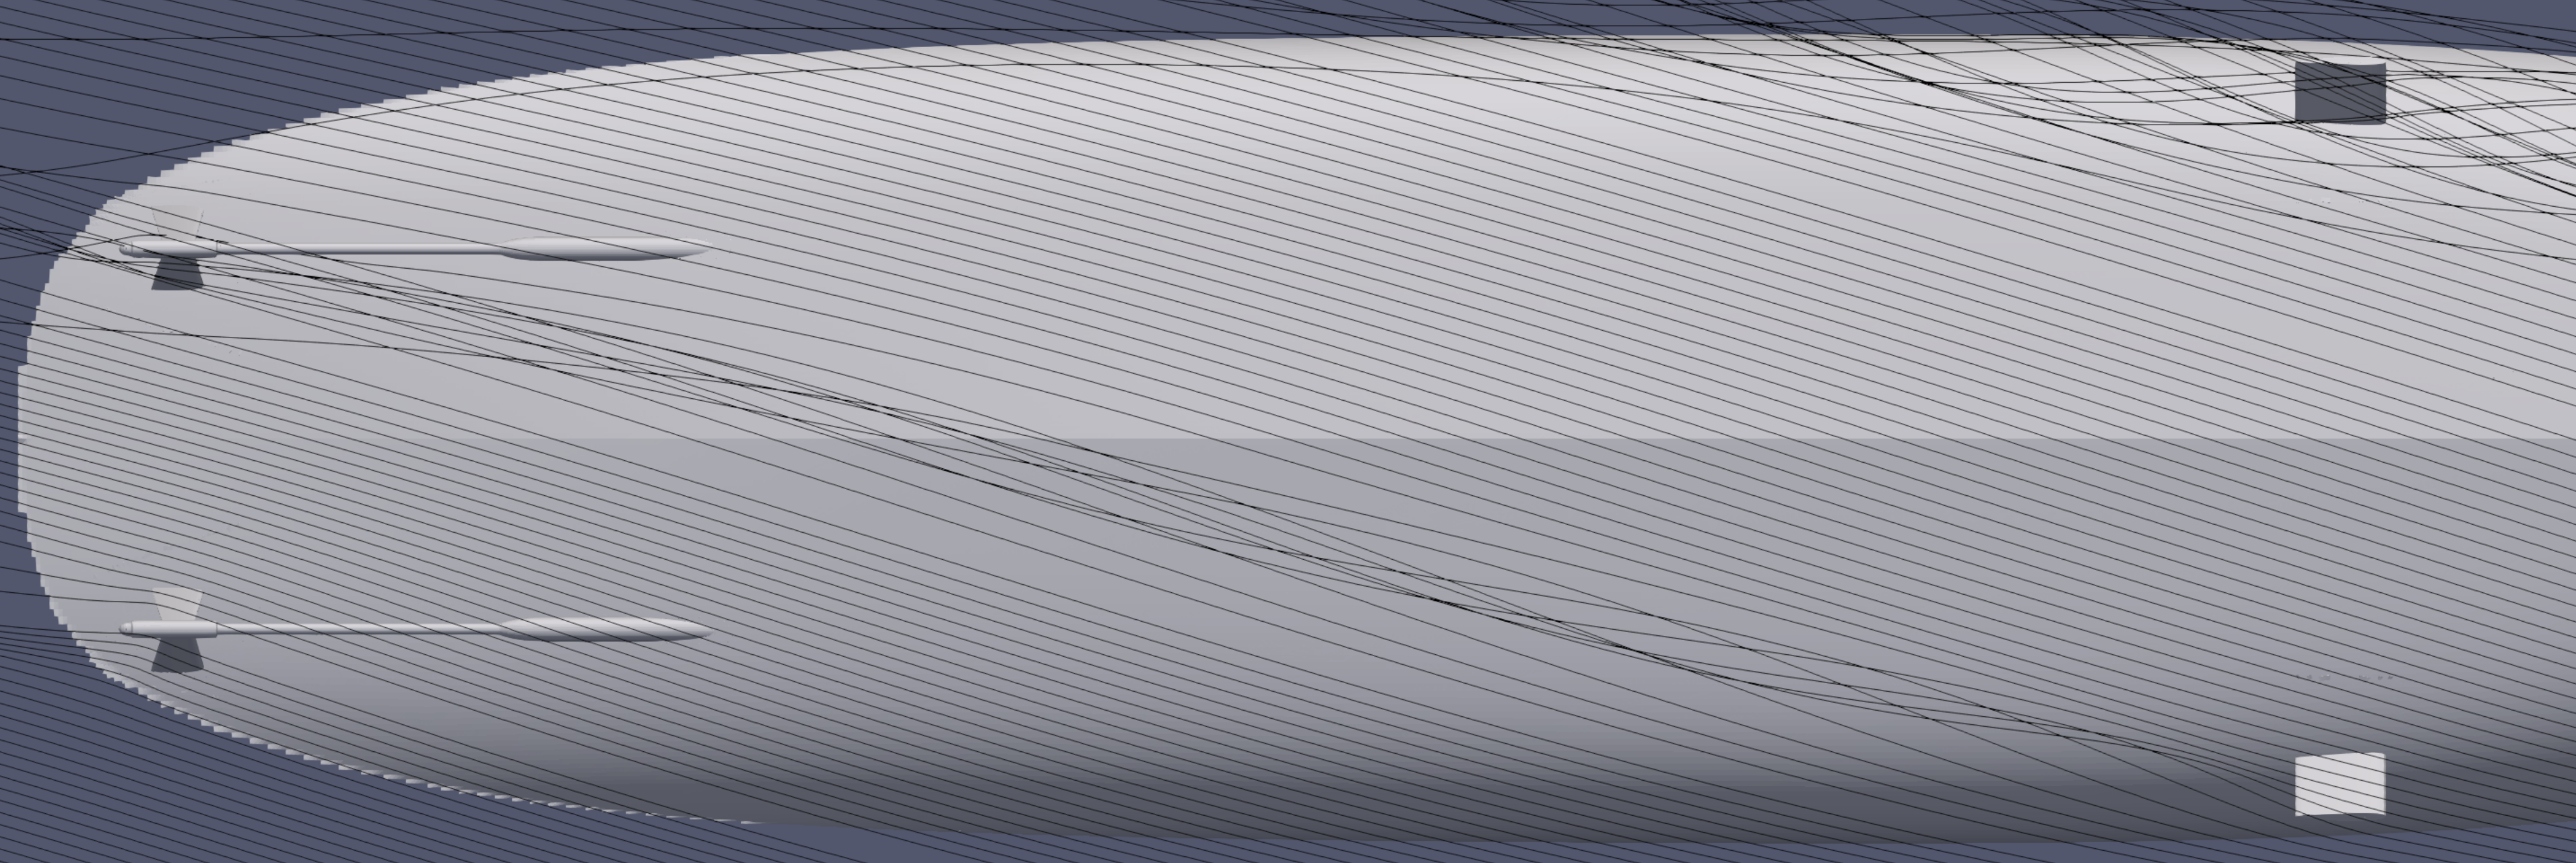
\includegraphics[width=\textwidth]{figures/paraview_drift_15.png}
    \caption{Streamlines for wPCC at 15 degrees drift angle.}
    \label{fig:streamlines15}
\end{figure}